
\documentclass{beamer}
\usecolortheme{dove}
\setbeamertemplate{navigation symbols}{}
\usepackage{amsmath,amssymb,amsfonts,amsthm, multicol, subfigure, color}
\usepackage{bm}
\usepackage{graphicx}
\usepackage{tabularx}
\usepackage{booktabs}
\usepackage{hyperref}
\usepackage{pdfpages}
\usepackage{xcolor}
\definecolor{seagreen}{RGB}{46, 139, 87}
\definecolor{mustard}{RGB}{234, 170, 0}
\def\independenT#1#2{\mathrel{\rlap{$#1#2$}\mkern2mu{#1#2}}}
\newcommand\indep{\protect\mathpalette{\protect\independenT}{\perp}}
\def\log{\text{log}}
\newcommand\logit{\text{logit}}
\newcommand\iid{\stackrel{\text{iid}}{\sim}}
\newcommand\E{\text{E}}
\newcommand\V{\text{V}}
\renewcommand\P{\text{P}}
\newcommand{\Cov}{\text{Cov}}
\newcommand{\Cor}{\text{Cor}}
\newcommand\doop{\texttt{do}}
\usepackage{stackrel}
\usepackage{tikz}
\usetikzlibrary{arrows,shapes.arrows,positioning,shapes,patterns,calc}
\newcommand\slideref[1]{\vskip .1cm \tiny \textcolor{gray}{{#1}}}
\newcommand\red[1]{\color{red}#1}
\newcommand\blue[1]{\color{blue}#1}
\newcommand\gray[1]{\color{gray}#1}
\newcommand\seagreen[1]{\color{seagreen}#1}
\newcommand\purple[1]{\color{purple}#1}
\newcommand\orange[1]{\color{orange}#1}
\newcommand\black[1]{\color{black}#1}
\newcommand\white[1]{\color{white}#1}
\newcommand\teal[1]{\color{teal}#1}
\newcommand\magenta[1]{\color{magenta}#1}
\newcommand\Fuchsia[1]{\color{Fuchsia}#1}
\newcommand\BlueGreen[1]{\color{BlueGreen}#1}
\newcommand\bblue[1]{\textcolor{blue}{\textbf{#1}}}
\newcommand\bred[1]{\textcolor{red}{\textbf{#1}}}
\newcommand\bgray[1]{\textcolor{gray}{\textbf{#1}}}
\newcommand\bgreen[1]{\textcolor{seagreen}{\textbf{#1}}}
\newcommand\bref[2]{\href{#1}{\color{blue}{#2}}}
\colorlet{lightgray}{gray!40}
\pgfdeclarelayer{bg}    % declare background layer for tikz
\pgfsetlayers{bg,main} % order layers for tikz
\newcommand\mycite[1]{\begin{scriptsize}\textcolor{darkgray}{(#1)}\end{scriptsize}}
\newcommand{\tcframe}{\frame{
%\small{
\only<1|handout:0>{\tableofcontents}
\only<2|handout:1>{\tableofcontents[currentsubsection]}}
%}
}

\newcommand{\goalsframe}{\begin{frame}{Learning goals for today}
By the end of class, you will be able to
\begin{itemize}
    \item connect causal inference\hfill (a missing data problem)\vskip .1in to statistical modeling\hfill (predicting missing data)
\end{itemize} \vskip .2in
\end{frame}}

\usepackage[round]{natbib}
\bibliographystyle{humannat-mod}
\setbeamertemplate{enumerate items}[default]
\usepackage{mathtools}

\title{Studying Social Inequality with Data Science}
\author{Ian Lundberg}
\date{\today}

\begin{document}

\begin{frame}
\begin{tikzpicture}[x = \textwidth, y = \textheight]
\node at (0,0) {};
\node at (1,1) {};
\node[anchor = north west, align = left, font = \huge] at (0,.9) {Studying\\Social Inequality\\with Data Science};
\node[anchor = north east, align = right] (number) at (1,.9) {INFO 3370 / 5371\\Spring 2023};
\node[anchor = north, font = \Large, align = left] at (.5,.5) {\bblue{Causal inference:}\\\bblue{Connections to statistical modeling}};
\end{tikzpicture}
\end{frame}

\goalsframe

\begin{frame}{A running example}

We should raise taxes on high earners to fund programs that seek to correct injustice \vskip .1in

\begin{itemize}
\item 1 = Agree
\item 0 = Disagree
\end{itemize} \vskip .3in \pause
What is the average causal effect of taking this class\\
on preferences for taxation to reduce injustice? \vskip .1in
\begin{itemize}
\item why might it be big?
\item why might it be small?
\item why is it hard to know the answer?
\end{itemize}

\end{frame}

\begin{frame}{Using potential outcomes}


\begin{tikzpicture}[x = \textwidth, y = .8\textheight]
\node at (0,0) {};
\node at (1,1) {};
\foreach \i in {.3, .4, .5,.6,.7,.8} {
	\draw[fill = blue, opacity = .3, color = blue] (.05,\i) rectangle (.25,\i + .1) {};
	\draw[fill = seagreen, opacity = .3, color = seagreen] (.25,\i) rectangle (.45,\i + .1) {};
}
\node[font = \footnotesize] at (.15,.85) {$Y_1^\text{Takes 3370}$};
\node[font = \footnotesize] at (.15,.75) {$Y_2^\text{Takes 3370}$};
\node[font = \footnotesize] at (.15,.55) {$Y_4^\text{Takes 3370}$};
\node[font = \footnotesize] at (.15,.65) {$Y_3^\text{Takes 3370}$};
\node[font = \footnotesize] at (.15,.45) {$Y_5^\text{Takes 3370}$};
\node[font = \footnotesize] at (.15,.35) {$Y_6^\text{Takes 3370}$};
\only<1>{
\node[font = \footnotesize] at (.35,.85) {$Y_1^\text{No 3370}$};
\node[font = \footnotesize] at (.35,.75) {$Y_2^\text{No 3370}$};
\node[font = \footnotesize] at (.35,.55) {$Y_4^\text{No 3370}$};
\node[font = \footnotesize] at (.35,.65) {$Y_3^\text{No 3370}$};
\node[font = \footnotesize] at (.35,.45) {$Y_5^\text{No 3370}$};
\node[font = \footnotesize] at (.35,.35) {$Y_6^\text{No 3370}$};
}
\only<2->{
\node[font = \footnotesize] at (.35,.85) {?};
\node[font = \footnotesize] at (.35,.75) {?};
\node[font = \footnotesize] at (.35,.55) {?};
\node[font = \footnotesize] at (.35,.65) {?};
\node[font = \footnotesize] at (.35,.45) {?};
\node[font = \footnotesize] at (.35,.35) {?};
}
\node[anchor = north, align = center, font = \footnotesize, blue] at (.15, .3) {Outcome\\under\\3370};
\node[anchor = north, align = center, font = \footnotesize, seagreen] at (.35, .3) {Outcome\\under\\no 3370};
\node[anchor = south, rotate = 90, align = center] at (.05, .6) {Each Row is a\\Student in This Class};
\node[anchor = north west, align = left, font = \footnotesize, align = left] at (.55,1) {$Y$ = We should raise taxes on\\high earners to fund programs\\that seek to correct injustice};
\node<3->[anchor = north west, align = left, align = left] at (.55,.6) {How could we learn\\about the (?)};
\end{tikzpicture}

\end{frame}

\begin{frame}{Strategy 1: People who nearly took the class} \pause

\begin{itemize}
\item Some of the class was on the waitlist
\begin{itemize}
\item some got in
\item others didn't
\end{itemize}
\end{itemize}

\end{frame}

\begin{frame}{Strategy 1: People who nearly took the class}


\begin{tikzpicture}[x = \textwidth, y = .8\textheight]
\node at (0,0) {};
\node at (1,1) {};
\foreach \i in {.1,.2,.3, .4, .5,.6,.7,.8} {
	\draw[fill = blue, opacity = .3, color = blue] (.05,\i) rectangle (.25,\i + .1) {};
	\draw[fill = seagreen, opacity = .3, color = seagreen] (.25,\i) rectangle (.45,\i + .1) {};
}
\node[font = \footnotesize] at (.15,.85) {$Y_1^\text{Takes 3370}$};
\node[font = \footnotesize] at (.15,.75) {$Y_2^\text{Takes 3370}$};
\node[font = \footnotesize] at (.15,.65) {$Y_3^\text{Takes 3370}$};
\node[font = \footnotesize] at (.15,.55) {$Y_4^\text{Takes 3370}$};
\node[font = \footnotesize] at (.15,.45) {?};
\node[font = \footnotesize] at (.15,.35) {?};
\node[font = \footnotesize] at (.15,.25) {?};
\node[font = \footnotesize] at (.15,.15) {?};
\node[font = \footnotesize] at (.35,.85) {?};
\node[font = \footnotesize] at (.35,.75) {?};
\node[font = \footnotesize] at (.35,.65) {?};
\node[font = \footnotesize] at (.35,.55) {?};
\node[font = \footnotesize] at (.35,.45) {$Y_5^\text{No 3370}$};
\node[font = \footnotesize] at (.35,.35) {$Y_6^\text{No 3370}$};
\node[font = \footnotesize] at (.35,.25) {$Y_7^\text{No 3370}$};
\node[font = \footnotesize] at (.35,.15) {$Y_8^\text{No 3370}$};
\draw<2->[fill = gray] (.47,.71) rectangle (.57,.89);
\node<2->[white, font = {\bf\scriptsize}, align = center] at (.52,.8) {Pre-\\Enroll};
\draw<2->[fill = gray] (.47,.31) rectangle (.57,.69);
\node<2->[white, font = {\bf\scriptsize}, align = center] at (.52,.5) {Waitlist};
\draw<2->[fill = gray] (.47,.11) rectangle (.57,.29);
\node<2->[white, font = {\bf\scriptsize}, align = center] at (.52,.2) {No\\Interest};
%\node[anchor = north, align = center, font = \footnotesize, blue] at (.15, .3) {Outcome\\under\\3370};
%\node[anchor = north, align = center, font = \footnotesize, seagreen] at (.35, .3) {Outcome\\under\\no 3370};
\node[anchor = south, rotate = 90, align = center] at (.05, .45) {Each Row is a\\Student in This Class};
\node[anchor = north west, align = left, font = \footnotesize, align = left] at (.6,1) {$Y$ = We should raise\\taxes on high earners\\to fund programs that\\seek to correct injustice};
\onslide<3->{
\draw[color = white, fill = white, fill opacity = .8] (.05,.1) rectangle (.6,.3);
\draw[color = white, fill = white, fill opacity = .8] (.05,.7) rectangle (.6,.9);
}
\node<4->[anchor = north west, align = left, font = \bf] (benefits) at (.6,.7) {Benefits of strategy};
\node<4->[anchor = north west, align = left, font = \bf] (drawbacks) at (.6,.5) {Drawbacks};
\node<5->[anchor = north west] at (benefits.south west) {Credible};
\node<5->[anchor = north west] at (drawbacks.south west) {Limited target population};
\end{tikzpicture}

\end{frame}

\begin{frame}{Strategy 1: People who nearly took the class}

Generalizing: Causal strategies in this domain \pause
\begin{itemize}
\item instrumental variables \pause
\item regression discontinuity \pause
\item interrupted time series \pause
\end{itemize} \vskip .2in
These strategies identify causal effects\\
by focusing on a feasible subpopulation\\
where treatment assignment is well-understood

\end{frame}

\begin{frame}

\begin{tikzpicture}[x = \textwidth, y = .8\textheight]
\node at (0,0) {};
\node at (1,1) {};
\foreach \i in {.3, .4, .5,.6,.7,.8} {
	\draw[fill = blue, opacity = .3, color = blue] (.05,\i) rectangle (.25,\i + .1) {};
	\draw[fill = seagreen, opacity = .3, color = seagreen] (.25,\i) rectangle (.45,\i + .1) {};
}
\node[font = \footnotesize] at (.15,.85) {$Y_1^\text{Takes 3370}$};
\node[font = \footnotesize] at (.15,.75) {$Y_2^\text{Takes 3370}$};
\node[font = \footnotesize] at (.15,.55) {$Y_4^\text{Takes 3370}$};
\node[font = \footnotesize] at (.15,.65) {$Y_3^\text{Takes 3370}$};
\node[font = \footnotesize] at (.15,.45) {$Y_5^\text{Takes 3370}$};
\node[font = \footnotesize] at (.15,.35) {$Y_6^\text{Takes 3370}$};
\only<1>{
\node[font = \footnotesize] at (.35,.85) {$Y_1^\text{No 3370}$};
\node[font = \footnotesize] at (.35,.75) {$Y_2^\text{No 3370}$};
\node[font = \footnotesize] at (.35,.55) {$Y_4^\text{No 3370}$};
\node[font = \footnotesize] at (.35,.65) {$Y_3^\text{No 3370}$};
\node[font = \footnotesize] at (.35,.45) {$Y_5^\text{No 3370}$};
\node[font = \footnotesize] at (.35,.35) {$Y_6^\text{No 3370}$};
}
\only<2->{
\node[font = \footnotesize] at (.35,.85) {?};
\node[font = \footnotesize] at (.35,.75) {?};
\node[font = \footnotesize] at (.35,.55) {?};
\node[font = \footnotesize] at (.35,.65) {?};
\node[font = \footnotesize] at (.35,.45) {?};
\node[font = \footnotesize] at (.35,.35) {?};
}
\node[anchor = north, align = center, font = \footnotesize, blue] at (.15, .3) {Outcome\\under\\3370};
\node[anchor = north, align = center, font = \footnotesize, seagreen] at (.35, .3) {Outcome\\under\\no 3370};
\node[anchor = south, rotate = 90, align = center] at (.05, .6) {Each Row is a\\Student in This Class};
\node[anchor = north west, align = left, font = \footnotesize, align = left] at (.55,1) {$Y$ = We should raise taxes on\\high earners to fund programs\\that seek to correct injustice};
\node[anchor = north west, align = left, align = left] at (.55,.6) {How could we learn\\about the (?)};
\end{tikzpicture}
\end{frame}


\begin{frame}{Strategy 2: Find your look-alikes on relevant dimensions} \pause

For each of you, we could compare
\begin{enumerate}
\item your opinion after 3370
\item the average opinion of non-3370 students who look like you
\end{enumerate} \pause
\vskip .3in
On what dimensions should they look like you?

\end{frame}

\begin{frame}{Strategy 2: Find your look-alikes on relevant dimensions}

Causal diagrams can help us reason about the adjustment set
\begin{itemize}
\item nodes are random variables
\item edges are causal relationships
\end{itemize}

\begin{center}
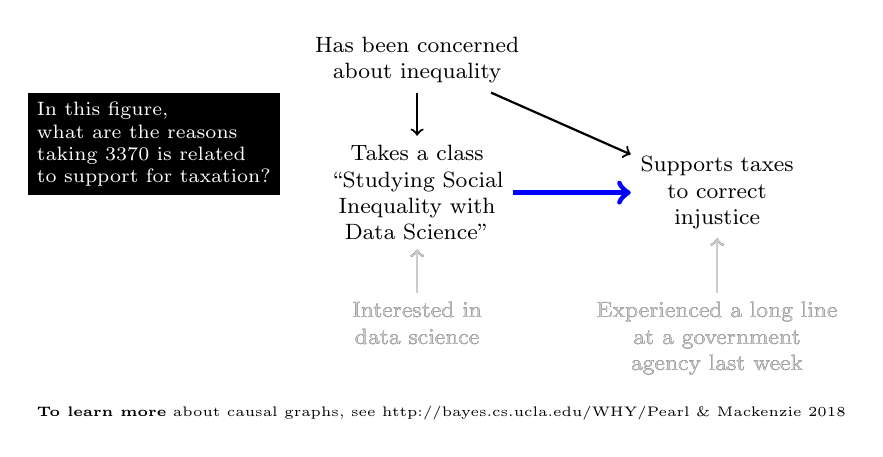
\begin{tikzpicture}[x = 1.5in, y = .5in]
\node[align = center, font = \footnotesize] (a) at (0,0) {Takes a class\\``Studying Social\\Inequality with\\Data Science''};
\node[align = center, font = \footnotesize] (y) at (1,0) {Supports taxes\\to correct\\injustice};
\draw[->, line width = 2pt, blue] (a) -- (y);
\onslide<2->{
\node[align = center, font = \footnotesize, anchor = south, align = center] (x) at (0,1) {Has been concerned\\about inequality};
\draw[->, thick] (x) -- (y);
\draw[->, thick] (x) -- (a);
}
\onslide<3-5>{
\node[align = center, font = \footnotesize, anchor = north, align = center] (e) at (1,-1) {Experienced a long line\\at a government\\agency last week};
\draw[->, thick] (e) -- (y);
}
\onslide<4-5>{
\node[align = center, font = \footnotesize, anchor = north, align = center] (z) at (0,-1) {Interested in\\data science};
\draw[->, thick] (z) -- (a);
}
\node<5->[anchor = north west, align = left, font  = \scriptsize, color = white, fill = black] at (-1.3,1) {In this figure,\\what are the reasons\\taking 3370 is related\\to support for taxation?};
\onslide<6>{
\node[align = center, font = \footnotesize, anchor = north, align = center, lightgray] (e) at (1,-1) {Experienced a long line\\at a government\\agency last week};
\draw[->, thick, lightgray] (e) -- (y);
\node[align = center, font = \footnotesize, anchor = north, align = center, lightgray] (z) at (0,-1) {Interested in\\data science};
\draw[->, thick, lightgray] (z) -- (a);
}
\node[anchor = west, font = \tiny] at (-1.3,-2.2) {\textbf{To learn more} about causal graphs, see \href{http://bayes.cs.ucla.edu/WHY/}{Pearl \& Mackenzie 2018}};
\end{tikzpicture}
\end{center}

\end{frame}

\begin{frame}{Strategy 2: Find your look-alikes on relevant dimensions}

\textbf{Benefits}
\begin{itemize}
\item Full target population
\end{itemize} \vskip .2in
\textbf{Drawbacks}
\begin{itemize}
\item May be less credible than approaches like the waitlist
\end{itemize}

\end{frame}

\begin{frame}{Strategy 2: Generalizing to a model} \pause

Regression = Tool to predict data you don't see \pause
\begin{itemize}
\item we don't see your outcome without 3370
\end{itemize} \vskip .3in \pause
Causal assumption: On average, $$Y_\text{You}^\text{No 3370} \approx \E(Y_\text{Others}^\text{No 3370}\mid\text{Look like you})$$ \pause \vskip .2in
The right side can be modeled statistically
\end{frame}

\begin{frame}{Strategy 2: Generalizing to a model}

\begin{tikzpicture}[x = \textwidth, y = .9\textheight]
\node[anchor = west] at (.75,.5) {
\includegraphics{legend}};
\node<1>[anchor = west] at (0,.5) {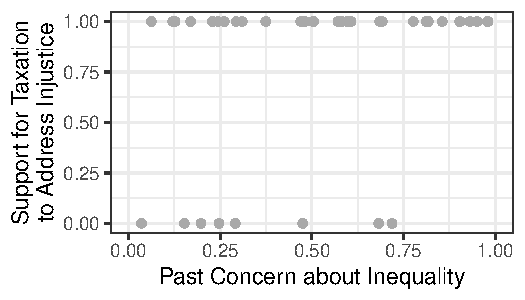
\includegraphics{p1}};
\node<2>[anchor = west] at (0,.5) {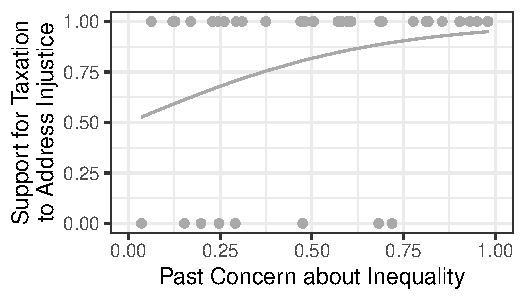
\includegraphics{p2}};
\node<3>[anchor = west] at (0,.5) {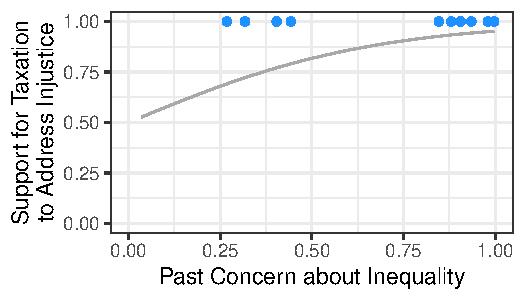
\includegraphics{p3}};
\node<4>[anchor = west] at (0,.5) {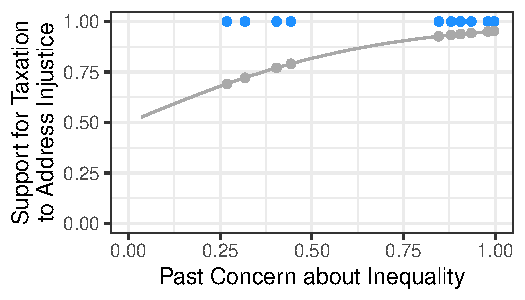
\includegraphics{p4}};
\node<5>[anchor = west] at (0,.5) {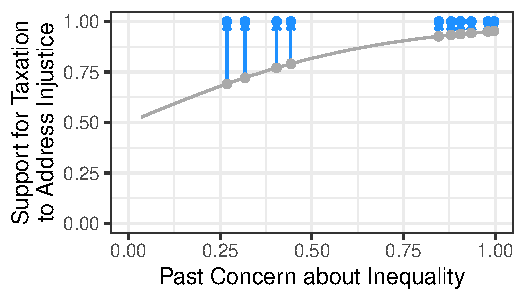
\includegraphics{p5}};
\node<1>[anchor = west] at (0,.1) {1) Find control units who didn't take this class};
\node<2>[anchor = west] at (0,.1) {2) Model their outcomes given pre-treatment variables};
\node<3>[anchor = west] at (0,.1) {3) Find the treated units of interest};
\node<4>[anchor = west] at (0,.1) {4) Predict their counterfactual outcomes};
\node<5>[anchor = west] at (0,.1) {5) Infer causal effect for each person. Average over people};
\end{tikzpicture}

\end{frame}

\begin{frame}{Strategy 2: Generalizing to a model}

\begin{tikzpicture}[x = \textwidth, y = .9\textheight]
%\node[anchor = west] at (.75,.9) {
\includegraphics{legend}};
\node[anchor = west] at (.75,.9) {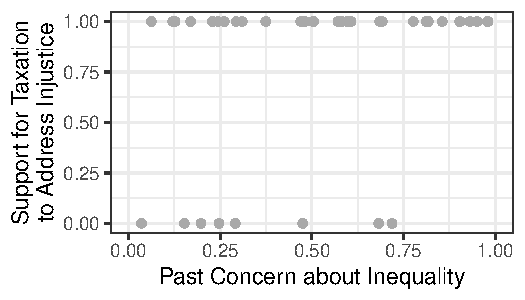
\includegraphics[scale = .3]{p1}};
\node[anchor = west] at (.75,.7) {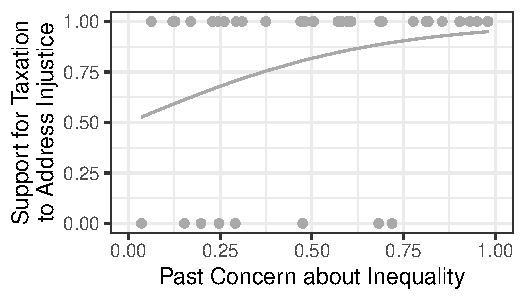
\includegraphics[scale = .3]{p2}};
\node[anchor = west] at (.75,.5) {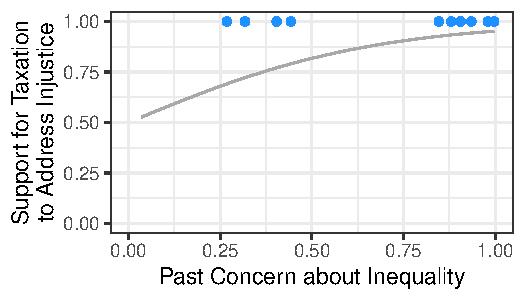
\includegraphics[scale = .3]{p3}};
\node[anchor = west] at (.75,.3) {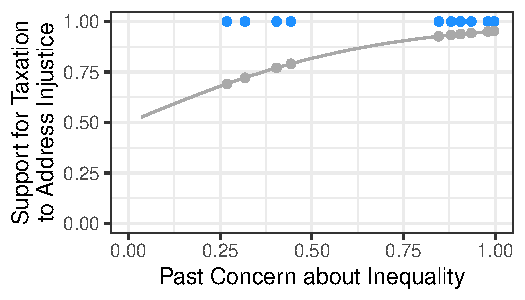
\includegraphics[scale = .3]{p4}};
\node[anchor = west] at (.75,.1) {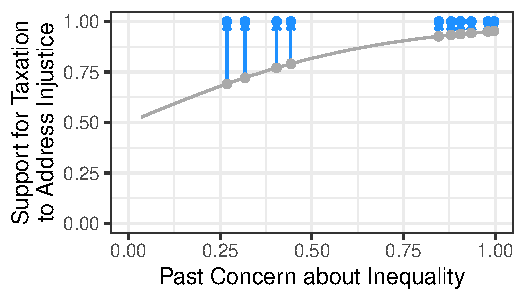
\includegraphics[scale = .3]{p5}};
\node[anchor = west, scale = .8] at (0,.9) {1) Find control units who didn't take this class};
\node[anchor = west, scale = .8] at (0,.7) {2) Model their outcomes given pre-treatment variables};
\node[anchor = west, scale = .8] at (0,.5) {3) Find the treated units of interest};
\node[anchor = west, scale = .8] at (0,.3) {4) Predict their counterfactual outcomes};
\node[anchor = west, scale = .8] at (0,.1) {5) Infer causal effect for each person. Average over people};
\end{tikzpicture}

\end{frame}

\begin{frame}{Summary: Causal inference is a missing data problem}


\begin{tikzpicture}[x = \textwidth, y = .8\textheight]
\node at (0,0) {};
\node at (1,1) {};
\foreach \i in {.3, .4, .5,.6,.7,.8} {
	\draw[fill = blue, opacity = .3, color = blue] (.05,\i) rectangle (.25,\i + .1) {};
	\draw[fill = seagreen, opacity = .3, color = seagreen] (.25,\i) rectangle (.45,\i + .1) {};
}
\node[font = \footnotesize] at (.15,.85) {$Y_1^\text{Takes 3370}$};
\node[font = \footnotesize] at (.15,.75) {$Y_2^\text{Takes 3370}$};
\node[font = \footnotesize] at (.15,.55) {$Y_4^\text{Takes 3370}$};
\node[font = \footnotesize] at (.15,.65) {$Y_3^\text{Takes 3370}$};
\node[font = \footnotesize] at (.15,.45) {$Y_5^\text{Takes 3370}$};
\node[font = \footnotesize] at (.15,.35) {$Y_6^\text{Takes 3370}$};
\only<1,3->{
\node[font = \footnotesize] at (.35,.85) {$Y_1^\text{No 3370}$};
\node[font = \footnotesize] at (.35,.75) {$Y_2^\text{No 3370}$};
\node[font = \footnotesize] at (.35,.55) {$Y_4^\text{No 3370}$};
\node[font = \footnotesize] at (.35,.65) {$Y_3^\text{No 3370}$};
\node[font = \footnotesize] at (.35,.45) {$Y_5^\text{No 3370}$};
\node[font = \footnotesize] at (.35,.35) {$Y_6^\text{No 3370}$};
}
\only<2>{
\node[font = \footnotesize] at (.35,.85) {?};
\node[font = \footnotesize] at (.35,.75) {?};
\node[font = \footnotesize] at (.35,.55) {?};
\node[font = \footnotesize] at (.35,.65) {?};
\node[font = \footnotesize] at (.35,.45) {?};
\node[font = \footnotesize] at (.35,.35) {?};
}
\node[anchor = north, align = center, font = \footnotesize, blue] at (.15, .3) {Outcome\\under\\3370};
\node[anchor = north, align = center, font = \footnotesize, seagreen] at (.35, .3) {Outcome\\under\\no 3370};
\node[anchor = south, rotate = 90, align = center] at (.05, .6) {Each Row is a\\Student in This Class};
\node<3->[anchor = north west] at (.52,.9) {\textbf{General approach}};
\node<4->[anchor = north west] at (.52,.8) {1) Define potential outcomes};
\node<5->[anchor = north west] at (.52,.72) {2) Define target population};
\node<6->[anchor = north west] at (.52,.64) {3) Make causal assumptions};
\node<7->[anchor = north west] at (.52,.56) {4) Model unobserved outcomes};
\node<8->[anchor = north west] at (.52,.48) {5) Predict them};
\node<9->[anchor = north west] at (.52,.4) {6) Report an average};
\end{tikzpicture}

\end{frame}

\begin{frame}

In what settings
\begin{itemize}
\item is it important to ask a causal question about inequality?
\item is it sufficient to ask a descriptive question?
\end{itemize}

\end{frame}

\goalsframe



\end{document}





